So far we have introduced the QAC language family for representing servers and
validators, and demonstrated the derivation mechanism with a $\Prog$ language.
Next I'll show how to prove that QAC validators are sound and complete:
\[\begin{array}{r@{\;}l}
\forall p:\Prog,&\letin{s}{\serverOf(p)}\\
&\letin{v}{\validatorOf(p)}\\
&\rejSound v s\wedge\rejComplete v s\\
&\text{\it i.e. }\forall t:\List(Q\times A),\\
&\qquad\valid s t\iff\accepts v t\\
&\qquad\text{\it i.e. }\exists s',\behaves s t s'\iff\exists v',\behaves v t v'
\end{array}\]

This section first presents a generic framework for proving validators'
correctness properties, and then demonstrates its usage by applying it to
$\Prog$-based validators.

\subsection{Proof strategy}
Both the specification and the validator are infinite loops, and the correctness
property is defined as equivalence between production and consumption of traces.
Therefore, we can prove this bisimulation relation by introducing some loop
invariant, and show that it is preserved in each step between the specification
and the validator.

\paragraph{Rejection soundness (acceptance completeness)}
To prove that any trace producible by server $\existT{S}{\sigma}{(\sstep,s_0)}$
is consumable by validator $\existT{V}{\beta}{(\vstep,v_0)}$, we need forward
induction on the server's execution path, and show that every step has a
corresponding validator step:
\begin{itemize}
\item The initial server state $s_0$ simulates the initial validator state $v_0$:
  \begin{equation}
    \tag{RejSound-Init}
    \label{eq:rs1}
    \Reflects{(v_0:\beta)}{(s_0:\sigma)}
  \end{equation}
\item Any server step $\sstep(q,c,s)=(a,s')$ whose pre-execution state $s$
  reflects some pre-validation state $v$ can be consumed by the validator
  into a post-validation state $v'$ that reflects the post-execution state $s'$:
  \begin{align*}
    \tag{RejSound-Step}
    \label{eq:rs2}
    &\forall(q:Q)(c:C)(a:A)(s,s':\sigma)(v:\beta),\\
    &\sstep(q,c,s)=(a,s')\wedge\Reflects{v}{s}\\
    &\implies\exists v':\beta,\vstep(q,a,v)=\Some{v'}\wedge\Reflects{v'}{s'}
  \end{align*}
  \begin{center}
    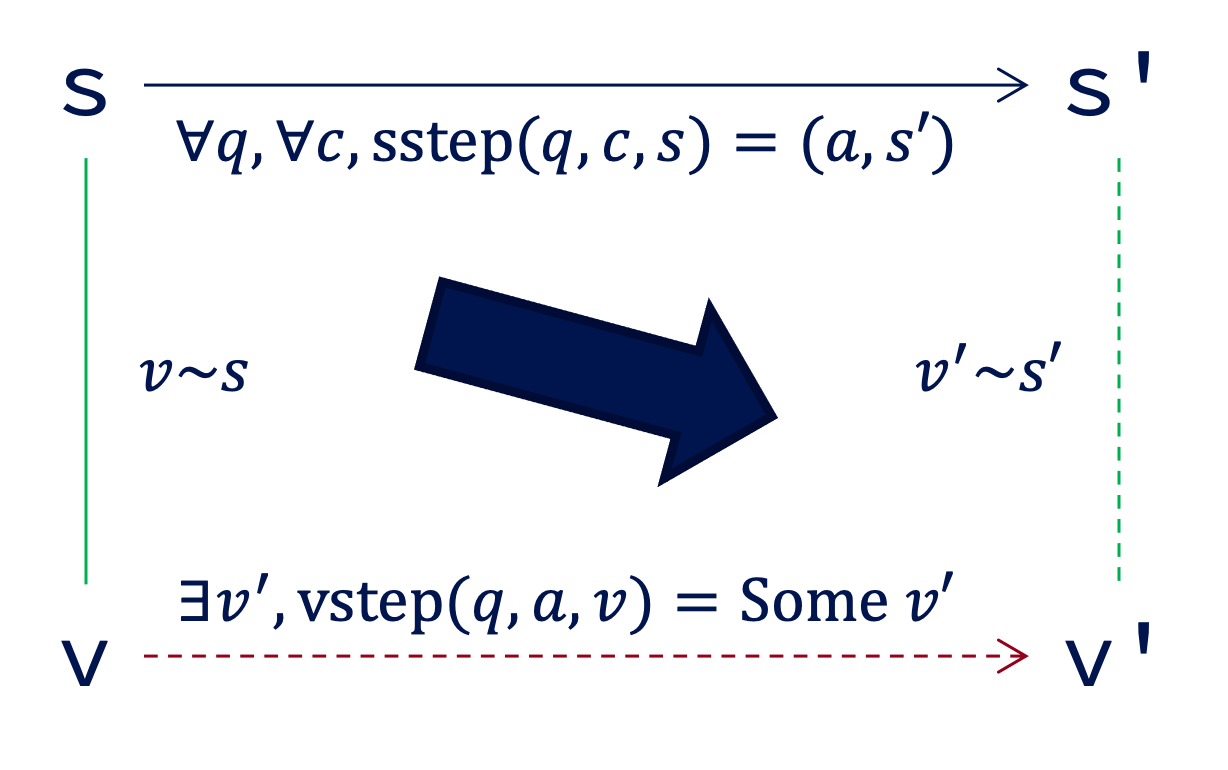
\includegraphics[width=.5\textwidth]{figures/sound}
  \end{center}
\end{itemize}

\paragraph{Rejection completeness (acceptance soundness)}
To prove that any trace consumable by validator
$\existT{V}{\beta}{(\vstep,v_0)}$ is producible by server
$\existT{S}{\sigma}{(\sstep,s_0)}$, we need backward induction on the
validator's execution path, and show that every step has a corresponding server
step:
\begin{itemize}
\item Any accepting validator step $\vstep(q,a,v)=\Some v'$ has some server
  state $s'$ that reflects the post-validation state $v'$:
  \begin{align*}
    \tag{RejComplete-End}
    \label{eq:rc1}
    \forall(q:Q)(a:A)(v, v':\beta),\;&\vstep(q,a,v)=\Some{v'}\\
    &\implies\exists s':\sigma,\Reflects{v'}{s'} 
  \end{align*}
\item Any accepting validator step $\vstep(q,a,v)=\Some v'$ whose
  post-validation state $v'$ reflects some post-execution server state $s'$
  has a corresponding server step from a pre-execution state $s$
  that reflects the pre-validation state $v$:
  \begin{align*}
    \tag{RejComplete-Step}
    \label{eq:rc2}
    &\forall(q:Q)(a:A)(v,v':\beta)(s':\sigma),\\
    &\vstep(q,a,v)=\Some{v'}\wedge\Reflects{v'}{s'}\\
    &\implies\exists(s:\sigma)(c:C),\sstep(q,c,s)=(a,s')\wedge\Reflects{v}{s}
  \end{align*}
  \begin{center}
    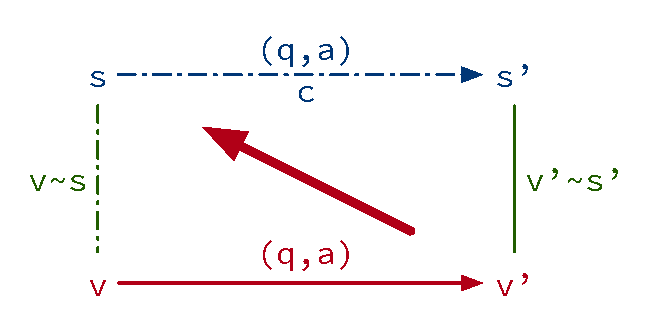
\includegraphics[width=.5\textwidth]{figures/complete}
  \end{center}

\item The initial validator state $v_0$ only reflects the initial server state $s_0$:
  \begin{equation}
    \tag{RejComplete-Init}
    \label{eq:rc3}
    \{s\mid\Reflects{v_0}{s}\}=\{s_0\}
  \end{equation}
\end{itemize}

Rejection soundness is proven by forward induction, while rejection completeness
is proven by backward induction.  This is because the choice $C$ is known from
the server step, but unknown from the validator step: Given a validator step, we
cannot predict ``what choices the server will make in the future'', but can
analyze ``what choices the server might have made in the past''.  This proof
strategy is further explained with the $\Prog$ example.

\subsection{Case study: Proving $\Prog$-based validators' correctness}
For specifications written in the $\Prog$ language, the validator is derived by
dualizing the server model.  It maintains a set of validation states, each state
corresponds to a possible execution path of the model program.

A validation state is accepting if its constraints are satisfiable, {\it i.e.}
there exists an assignment of the symbolic variables that can unify the trace
with the server model.

The validator accepts the trace if any of its validation states is accepting,
which indicates that some execution path of the server model can produce the
trace.

Given an accepting validation state, we can construct the server steps that
produce the trace, using the assignment $(\Var\to\Int)$ that satisfies the
constraints.  This assignment evaluates internal choices' symbolic variables
into concrete values, and evaluates the validator's key-variable mapping
$(\Nat\to\Var)$ to the server's key-value mapping $(\Nat\to\Int)$.

Therefore, we only need to show that each server and validator step preserves
the existence of such assignment that relates their states.

For the rest of this section, $\beta=\Set((\Nat\to\Var)\times\Set\constraint)$
represents the validator state type, and $\sigma=\Nat\to\Int$ represents the
server state type.

\begin{definition}[Invariant between $\Prog$-based specification and validator]
  Validator state $v$ simulates server state $s$ if it contains a validation
  state $(vs,cs)$ that {\em reflects} the server state, {\it i.e.}  (1) There
  exists an assignment $asgn$ that can satisfy the constraints $cs$; and (2) The
  key-variable mapping $vs$ can be evaluated with $asgn$ (written as
  $vs^{asgn}$) into a key-value mapping that is equivalent with
  $s$: \[\begin{array}{lll} \Reflects{(v:\beta)}{(s:\sigma)}&\triangleq& \exists((vs,cs)\in
  v)(asgn:\Var\to\Int),\satisfy{asgn} cs\wedge vs^{asgn}\equiv s\\
  vs^{asgn}&\triangleq&addr\mapsto asgn!(vs!addr) \end{array}\]
\end{definition}

\begin{lemma}[\ref{eq:rs1}]
\[\begin{array}{ll}
\text{If:}&
vs=(\_\mapsto\#0)\qquad
cs=\{\#0\equiv0\}\qquad
s=(\_\mapsto0)\\
\text{Then:}&\Reflects{\{(vs,cs)\}}{s}
\end{array}\]
\end{lemma}
\begin{proof}
Since $(vs,cs)$ is the only element in the validator state, we only need to show
that:
\[\exists(asgn:\Var\to\Int),\satisfy{asgn} cs\wedge vs^{asgn}\equiv s\]

By constructing the assignment as: \[asgn=(\_\mapsto0)\]

We have: \[\#0^{asgn}=0\]

Thus: \[\satisfy{asgn} cs\]

We also know that: \[\forall k, asgn!(vs!k)=0=(s!k)\]

Thus: \[vs^{asgn}\equiv s\]
\end{proof}

\begin{lemma}[\ref{eq:rs2}]
  \begin{align*}
    &\forall(p:\Prog)(q,c,a:\Int)(s,s':\sigma)(v:\beta),\\
    &\sstep_p(q,c,s)=(a,s')\wedge\Reflects{v}{s}\\
    &\implies\exists v':\beta,\vstep_p(q,a,v)=\Some{v'}\wedge\Reflects{v'}{s'}
  \end{align*}
\begin{proof}
The invariant $\Reflects{v}{s}$ tells us that $v$ contains a validation state
that reflects the server state $s_0$:
\[\exists(vs,cs)\in v,\exists asgn:\Var\to\Int,\quad\satisfy{asgn} cs\wedge {vs}^{asgn}\equiv s\]

Since the server's internal choice was provided, we can compute the server's
actual execution path.  For each small step of the server's execution, we can
construct its corresponding validator small step, based on the derivation rules
in \autoref{sec:dualization}.  By making the same internal choice and branch
decisions as the server did, we can construct the assignment that unifies the
validator with the server.  The proof details are shown in \autoref{sec:rs2-proof}.
\end{proof}
\end{lemma}

\begin{lemma}[\ref{eq:rc1}]
\begin{align*}
\forall(p:\Prog)(q,a:\Int)(v,v':\beta),\;&\vstep_p(q,a,v)=\Some{v'}\\
&\implies\exists s':\sigma,\Reflects{v'}{s'}
\end{align*}
\begin{proof}
Since $\vstep_p$ checks the nonemptiness of the result, we know that $v'$ must
be nonempty.  Consider validation state $(vs',cs')\in v'$.  Since $\vstep'_p$
checks that $(\solvable cs')$, we know that:
\[\exists asgn,\quad\satisfy{asgn}cs'\]

Let:
\[s'=vs'^{~asgn}\]

Then we have:
\begin{align*}
&(vs',cs')\in v'\wedge \satisfy{asgn}{cs'}\wedge vs'^{~asgn}\equiv s'\\
&\textit{i.e. }\Reflects{v'}{s'}
\end{align*}
\end{proof}
\end{lemma}

\begin{lemma}[\ref{eq:rc2}]
\begin{align*}
&\forall(p:\Prog)(q,a:\Int)(v,v':\beta)(s':\sigma),\\
&\vstep_p(q,a,v)=\Some{v'}\wedge\Reflects{v'}{s'}\\
&\implies\exists(s:\sigma)(c:\Int),\sstep_p(q,c,s)=(a,s')\wedge\Reflects{v}{s}
\end{align*}
\begin{proof}
We first construct the initial server state $(s:\sigma\mid\Reflects{v}{s})$.  We
then compute the internal choice $c$ and construct the server step that
corresponds with the validator step.

The definition of $\Reflects{v'}{s'}$ says:
\[\exists (vs',cs')\in v',\exists asgn,\quad \satisfy{asgn}{cs'}\wedge vs'^{~asgn}\equiv s'\]

From the definition of $\vstep_p$, we know that:
\[\exists (vs,cs)\in v,\quad \vstep'_p(q,a,(vs,cs))=(vs',cs')\]

Since $\vstep'_p$ monotonically increases set of constraints, we have
$cs\subseteq cs'$.  Therefore: \[\satisfy{asgn}{cs}\]

Let: \[s=vs^{asgn}\]

Then we have:
\begin{align*}
&(vs,cs)\in v\wedge\satisfy{asgn}{cs}\wedge vs^{asgn}\equiv s\\
&\textit{i.e. }\Reflects{v}{s}
\end{align*}

From the definition of $\vstep'_p$, the validator first creates a fresh variable
to represent the server's internal choice.  Let:
\[x_c=\Fresh(vs,cs)\qquad c=asgn!x_c\]

We now have a server step $\sstep_p(q,c,s)$, and need to show that it results in
response $a$ and post-execution state $s'$.  Since the post-validation state
$v'$ simulates $s'$ and guarantees the response to be $a$, we only need to show
that the server step is reflected in the validator.  This is done by analyzing
the server's execution path, proving that each derivation rule preserves such
small-step reflection.  The proof details are shown in \autoref{sec:rc2-proof}
\end{proof}
\end{lemma}

\begin{lemma}[\ref{eq:rc3}]
\[\begin{array}{ll}
\text{If:}&
vs=(\_\mapsto\#0)\qquad
cs=\{\#0\equiv0\}\qquad
s_0=(\_\mapsto0)\\
\text{Then:}&\{s\mid\Reflects{\{(vs,cs)\}}{s}\}=\{s_0\}
\end{array}\]
\begin{proof}
The requirement for $s$ says:
\[\exists asgn:\Var\to\Int,\quad\satisfy{asgn}{cs}\wedge vs^{asgn}=s\]

The constraint satisfaction tells us that:
\[asgn!0=0\]

We then have:
\[\forall k:\Nat,\quad s!k=asgn!(vs!k)=asgn!0=0=s_0!k\]

Therefore, $s_0$ is the only server state that $(vs,cs)$ simulates.
\end{proof}
\end{lemma}

So far, we've proven the soundness and completeness of all validators derived
from the $\Prog$ language.  The main idea is to show the reflection between the
server and the validator, by constructing the assignments that unifies them.

This also answers why proving rejection completeness requires backward
induction: The assignment evaluates the symbolic variables during the validation
process, which includes all choces made by the server, past and future.  An
assignment might include wrong predictions about the server's future choices, in
which case the validator will drop it upon contradicting observations.  By the
end of validation, the surviving assignment can let us reconstruct a server's
execution path, by infering its internal choices.
